Charged particles that move through the solenoidal magnetic field that surrounds
the ATLAS tracking system, follow helical trajectories. The projection of a
helix on the $xy$ plane is a circle and, in order to uniquely parametrize the
particle track in three dimensions, five parameters are needed. A common choice
is to use the \emph{perigee} parameters, where the perigee is the point of
closest approach to the beam axis. With this choice, the five parameters are:
\begin{itemize}
\item The signed curvature $C$ of the helix, defined as $C = q / 2R$ where $q$
  is the particle charge and $R$ is the radius of the helix. This is related to
  the transverse momentum $\pt = qB / C$, where $B$ is the magnetic field
  measured in Tesla, C is measured in m$^{-1}$ and $\pt$ in GeV.
\item The distance of closest approach $d_0$ in the $xy$ plane measured in
  millimeter.
\item The $z$ coordinate of the point of closest approach, denoted by $z_0$ and
  measured in millimeters.
\item The azimuthal angle $\phi_0$ of the tangent to this point.
\item The polar angle $\theta$ to the $z$-axis.
\end{itemize}
The perigee and the track parameters are schematized in
Figure~\ref{fig:track_par}.
\begin{figure}[!h]
  \centering
    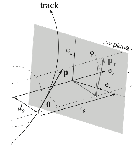
\includegraphics[width=.8\linewidth]{track_parameters}
    \caption{Track parameters at the perigee. In the figure \textbf{p} is the
      momentum of the incoming particle, e$_\mathrm{x}$, e$_\mathrm{y}$,
      e$_\mathrm{z}$ are the versors of the coordinate system defined in
      \cref{sec:coordinate-system} and $\theta$ and $\phi$, also defined in
      \cref{sec:coordinate-system} are the polar and azimuthal angle
      respectively.}
    \label{fig:track_par}
\end{figure}
%%% Local Variables:
%%% mode: latex
%%% TeX-master: "../search_for_DM_LED_with_ATLAS"
%%% End:
